%!TEX root = Digest.tex


% \begin{figure}[ht]
%     \centering
%     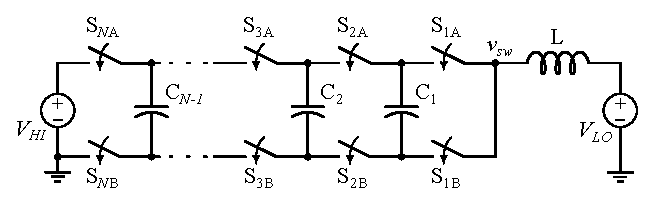
\includegraphics[width=0.5\linewidth]{Figures/FCML.eps}
%     \caption{Generic N-level FCML converter topology. }
%     \label{fig:schem}
% \end{figure}


\vspace{-15pt}
\section{Theory of Operation}
\vspace{-0.75em}
Figure \ref{fig:schem} shows a generic step-down $N$:\,1 FCML converter, where the input and output voltages are denoted as $V_{HI}$ and $V_{LO}$, respectively.
In this work, the parameter $N$ refers to both the conversion ratio of the FCML converter as well as the number of complementary switch-pairs, $S_{N\textrm{A/B}}$.
While the FCML converter can operate in resonance mode with fixed conversion ratios equal to or greater than $1/N$ (i.e., $N$:\,2, $N$:\,3, ...), this work will analyze the most extreme conversion ratio, $N$:1.

\begin{figure}[b]
\vspace{-5pt}
\centering
    \captionsetup{width=1\linewidth}\hspace{0pt}
    \hspace{-5pt}\subfloat[Generic $N$:1 FCML\label{fig:schem}]  {\hspace{0pt}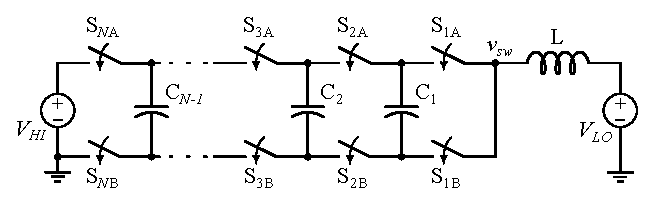
\includegraphics[width=0.4\linewidth]{Figures/FCML.eps}}
    \hspace{20pt}\subfloat[Phase 1\label{fig:Charge_ph1}]  {\hspace{0pt}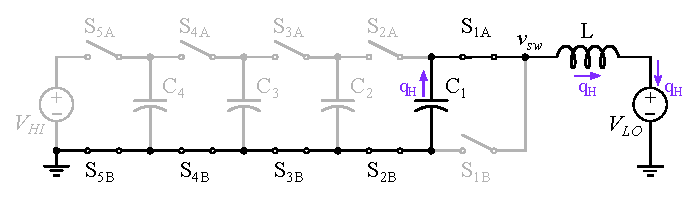
\includegraphics[width=0.4\linewidth]{Figures/FCML_ph1.eps}}\\
    \subfloat[Phase 2\label{fig:Charge_ph2}] {\hspace{0pt}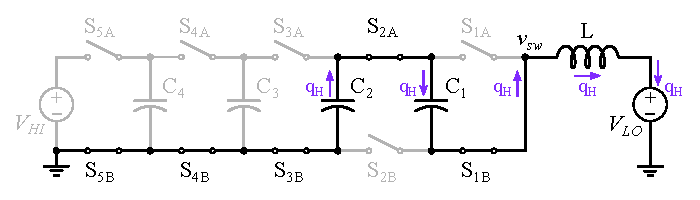
\includegraphics[width=0.4\linewidth]{Figures/FCML_ph2.eps}}
    \hspace{20pt}\subfloat[Phase 3\label{fig:Charge_ph3}]  {\hspace{0pt}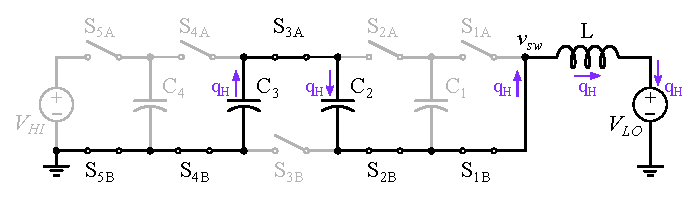
\includegraphics[width=0.4\linewidth]{Figures/FCML_ph3.eps}}\\
    \subfloat[Phase 4\label{fig:Charge_ph4}] {\hspace{0pt}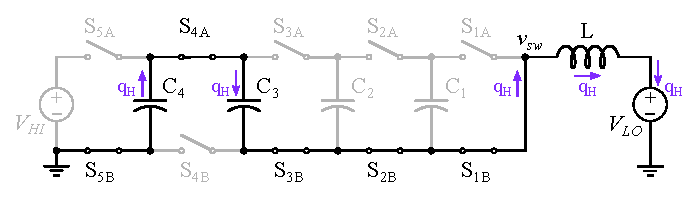
\includegraphics[width=0.4\linewidth]{Figures/FCML_phN-1.eps}}
   \hspace{20pt}\subfloat[Phase 5\label{fig:Charge_ph5}] {\hspace{0pt}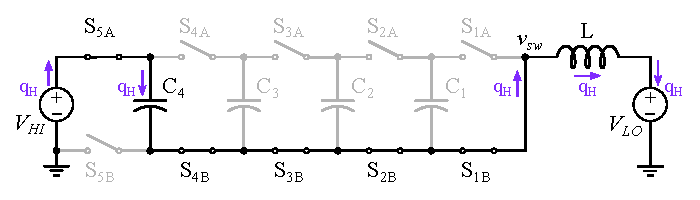
\includegraphics[width=0.4\linewidth]{Figures/FCML_phN.eps}}\\
    
    \caption{Schematic for (a) a generic $N$:\,1 FCML converter, and (b)-(f) a 5:1 FCML converter, highlighting the charge flow during each phase, normalized with respect to high-side input charge quantity $q_H$.} 
\label{fig:Charge}
% \vspace{-5pt}
\end{figure}


%When operating in regulation mode, phase-shifted pulse width modulation (PS-PWM) is often used to control the switches as it results in natural balancing of the flying capacitor voltages \textcolor{blue}{cite something here about PS-PWM balancing}. However, PS-PWM does not allow for resonant operation and therefore a new switch timing method must be analyzed which allows for both capacitor balancing as well as resonance mode operation. While the N-level FCML converter can be operated as a fixed-ratio converter with conversion ratios equal to N:1, (N-1):1, (N-2):1...1:1 depending on configuration, this work will focus on the most extreme conversion ratio, N:1.





%- In this paper, ``$N$" refers to the number of switch-pairs (and to the fixed-conversion ratio mentioned later?). There are $N-1$ flying capacitors

%-Slight variation to the typical (?) PSPWM 

%- in PSWPM at a ``special" duty cycle that is an integer multiple of $1/N$, each state produces the same voltage at the switch node, i.e (ignoring capacitor ripple) switch-node voltage is constant and the FCML operates as a fixed-ratio converter

%-  Here, just look at the lowest ``special" duty cycle regime, i.e. $0 \text{ -- } 1/N \%$ (a citation about duty cycle ranges?) because? high conversion ratio reason???

The gate timings of each switch pair, as shown in Fig.~\ref{fig:gate_signals}, are adjusted to ensure half-sine-wave (resonant) or a symmetric sine-wave segment (above resonance) inductor current in each phase, as illustrated in Fig.~\ref{fig:iL_freq}.
% \cite{Schaef_TPEL2018}
% Example gate timings are illustrated in Fig.~\ref{fig:gate_signals}.
To determine appropriate phase durations, charge flow analysis is performed ~\cite{Seeman2008}.
%, as well as, charge balancing. 
While this analysis is suitable for any $N$:1 FCML, Fig.~\ref{fig:Charge} depicts the circuit schematics for each phase of an example 5:1 step-down FCML converter where the charge $q_{H}$ is defined as the product of the average current supplied by the high-side voltage, $V_{HI}$, and the switching period: $q_{H} = I_{HI}\cdot T_{\textrm{sw}}$.
Phase 5 (Fig.~\ref{fig:Charge_ph5}) is the only phase in which $V_{HI}$ is connected, therefore, the charge supplied by $V_{HI}$ in this phase must equal $q_{H}$.

Following the charge flow across phases, each flying capacitor is charged by $q_{H}$ in one phase and discharged by $q_{H}$ in one other phase, thereby maintaining charge balance across the capacitors in periodic steady-state.
Because each flying capacitor is charged/discharged by the same charge quantity, equating all capacitances $C_1 \text{ -- } C_{N-1}$ to an equivalent value, $C_{0}$, enforces equivalent voltage ripple magnitude on each of the flying capacitors.
%- \textcolor{red}{[Not sure if we need to include this] Continuing charge flow analysis, the total charge delivered to the low-side voltage, $V_{LO}$, is equal to the summation of charge delivered through the inductor, $L$, during each phase. For a resonant FCML, (or something like: For an FCML operated in this way?) one $q_{HI}$ quantity is delivered during each of the five phases (\textit{N} phases), making the sum equal to $q_{LO} = Nq_{HI}$. The fixed conversion ratio is calculated as a ratio of the high-side charge to the low-side charge, i.e. $q_{HI}/q_{LO} = 1/N$.}
Finally, one $q_{H}$ quantity is delivered to the low-side voltage, $V_{LO}$ through inductor $L$ during each of the five phases (\textit{N} phases).
% \textcolor{red}{The consequent phase durations needed for successful resonant (and above-resonant) operation are calculated by ensuring this charge balance between phases of the inductor current.}




% \begin{figure}
% \vspace{-20pt}
% \centering
%     \captionsetup{width=1\linewidth}\hspace{0pt}
%     \subfloat[Phase 1.\label{fig:Charge_ph1}]  {\hspace{0pt}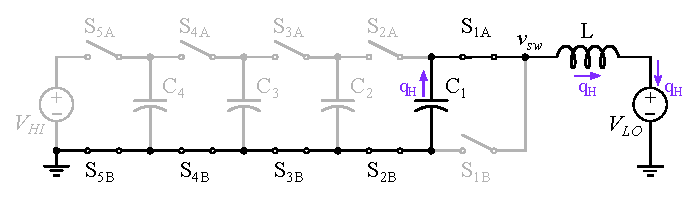
\includegraphics[width=0.4\linewidth]{Figures/FCML_ph1.eps}}
%     \hspace{20pt}\subfloat[Phase 2.\label{fig:Charge_ph2}] {\hspace{0pt}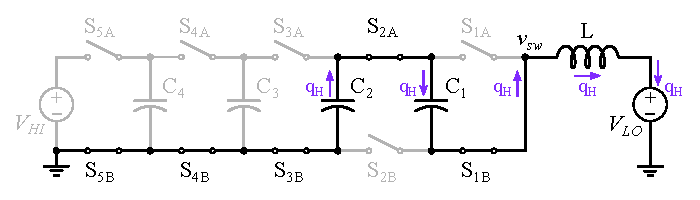
\includegraphics[width=0.4\linewidth]{Figures/FCML_ph2.eps}}\\
%     \subfloat[Phase 3.\label{fig:Charge_ph3}]  {\hspace{0pt}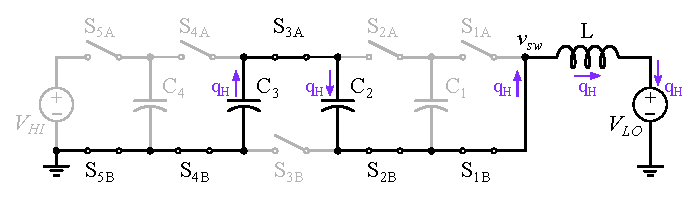
\includegraphics[width=0.4\linewidth]{Figures/FCML_ph3.eps}}
%     \hspace{20pt}\subfloat[Phase 4.\label{fig:Charge_ph4}] {\hspace{0pt}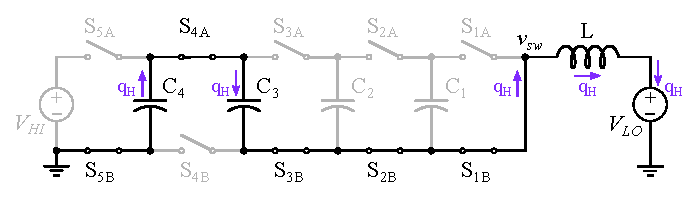
\includegraphics[width=0.4\linewidth]{Figures/FCML_phN-1.eps}}\\
%   \hspace{20pt}\subfloat[Phase 5.\label{fig:Charge_ph5}] {\hspace{0pt}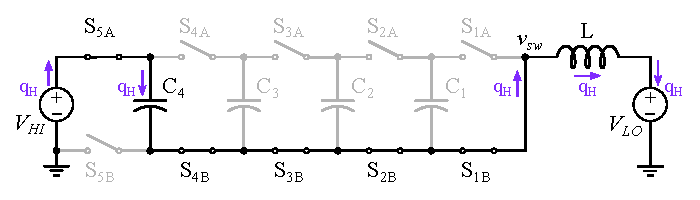
\includegraphics[width=0.4\linewidth]{Figures/FCML_phN.eps}}
    
%     \caption{Circuit states for a 5-level FCML converter, highlighting the charge flow during each sub-phase.} 
% \label{fig:Charge}
% \end{figure}


\vspace{-10pt}
\section{Calculating Phase Durations}
\vspace{-0.75em}
To calculate ideal timing durations of each phase in periodic steady-state, the inductor current is assumed to start and end each phase at the same value, implying zero net volt-seconds across the inductor within each phase and minimized rms current ripple within a total period for reduced conduction and ac losses.
Furthermore, for this analysis a high Q-factor is reasonably assumed for each phase configuration, leading to sinusoidal behavior with negligible damping.


% \begin{align}
%     q_{1}\cdot t_{1} = I_{1}\\
%     q_{2}\cdot t_{2} = I_{2}
%     \label{eqn:atres_q}
% \end{align}

\begin{figure}[t]
\vspace{-25pt}
\begin{minipage}[H]{0.45\linewidth}
    \centering
    \vspace{8pt}
    % 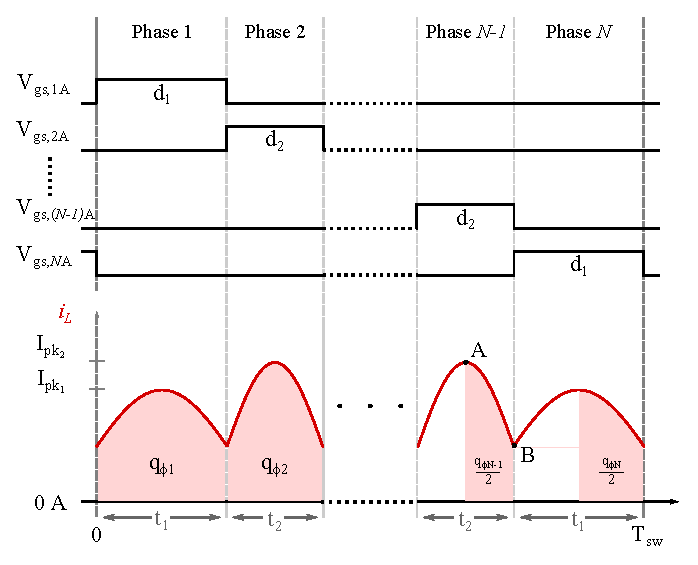
\includegraphics[width=1\linewidth]{Figures/FCML_gate1.eps} % With quarter-wave symmetry
    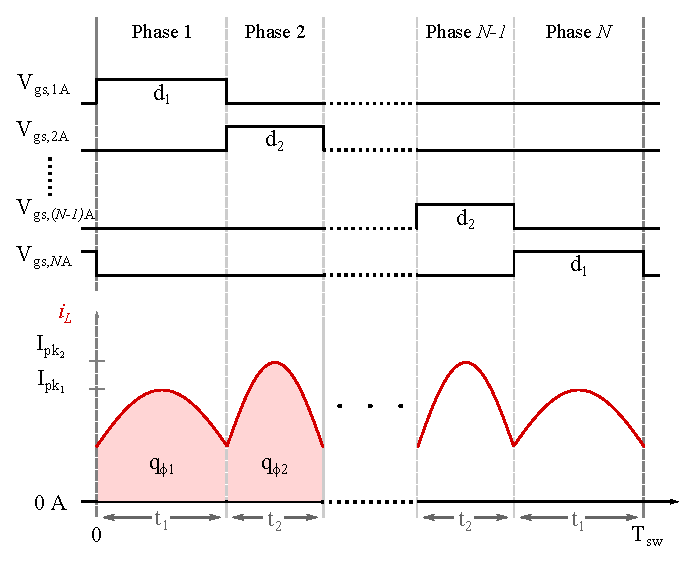
\includegraphics[width=1\linewidth]{Figures/FCML_gate2.eps} % Without quarter-wave symmetry
    \caption{Modulation scheme at- and above-resonance for $N$:1 FCML. The current $i_{L}$ is shown for above-resonance.}
    \label{fig:gate_signals}
\end{minipage}
\hspace{20pt}
\begin{minipage}[H]{0.45\linewidth}
    \centering
    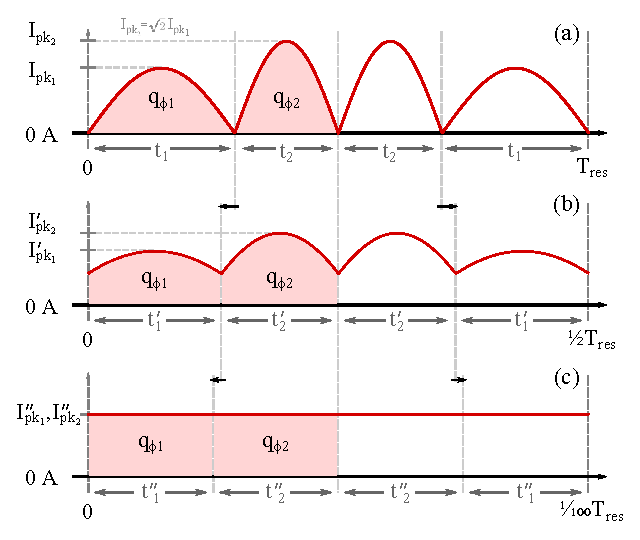
\includegraphics[width=1\linewidth]{Figures/iL_freq_range.eps}
    \caption{Example 4:1 FCML inductor current waveforms at (a) $\Gamma=1$, (b) $\Gamma=0.5$, and (c) $\Gamma=0.01$.}
    \label{fig:iL_freq}
\end{minipage}
\vspace{-10pt}
\end{figure}



\vspace{-10pt}
\subsection{At Resonance {\normalfont ($\Gamma=1$)}}
\vspace{-0.75em}
% There are a few constraints on the system that will allow us to determine the on-times of each state for general above resonance operation.

%The equivalent circuits for phase 1 and phase $N$ are the same, as shown in Fig. \ref{fig:Charge_ph1} and Fig.\ref{fig:Charge_ph5}.
%Only one flying capacitor with capacitance $C_0$ is connected in series with the inductor, therefore the resonant frequency $\omega_{r1}$ for phase 1 and phase $N$ can be calculated using~(\ref{eqn:omega_r1}).

As shown in Fig. \ref{fig:Charge_ph1} and Fig.\ref{fig:Charge_ph5}, only one flying capacitor with capacitance $C_0$ is connected in series with the inductor during phase 1 and phase $N$, allowing their resonant frequency, $\omega_{r1}$, to be calculated using~(\ref{eqn:omega_r1}).


Similarly, all other phases ($2, 3,...,N\textrm{-}1$) are topologically equivalent, as they have two series-connected flying capacitors connected with the inductor. The resonant frequency in these phases can therefore be calculated using (\ref{eqn:omega_r2}).
The relationship between the two resonant frequencies can be found as shown in (\ref{eqn:omega_r1_to_r2}).
Since equal charge $q_H$ flows through the inductor during each phase ($q_{H} = I_{L,\textrm{avg}_i}\cdot t_{\phi_i}$), the relationship between the peak inductor currents, $I_{\textrm{pk}_1}$ and $I_{\textrm{pk}_2}$, during each phase is determined by their resonant frequency ratio, yielding $\sqrt{2}\ I_{\textrm{pk}_1} = I_{\textrm{pk}_2}$. Example inductor current waveforms while operating at resonance can be seen in Fig. \ref{fig:iL_freq}a.



%The resonant frequency $\omega_{r1}$ of the first resonant phase, as depicted in Fig. \ref{fig:Charge_ph1}, where one flying capacitor $C_0$ is connected in series with the inductor in (\ref{eqn:omega_r1}) and 
%in  are used to derive a fixed relationship between the resonant frequencies as shown in .

%- Mention effective capacitance per phase and reference Fig.~\ref{fig:Charge}

%- Mention that phase 1, phase N equivalent. and phase 2,3..N-1 equivalent and therefore same timings and same peaks

\centerline{
% \vspace{-5pt}
\begin{tabular}{cccc}
    \hspace{-20pt}
    \noindent
    \parbox[c]{0.22\textwidth}{
    	\begin{equation}
        	\omega_{r1} = \frac{1}{\sqrt{L C_0}}
        	\label{eqn:omega_r1}
    	\end{equation}
    }
    &
    \begin{minipage}{0.27\textwidth}
    	\begin{equation}
    	    \omega_{r2} = \frac{1}{\sqrt{L\cdot \bigl(\frac{1}{2} C_0 \bigr)}}
        	\label{eqn:omega_r2}
    	\end{equation}
    \end{minipage}
    &
    \noindent\parbox[c]{0.22\textwidth}{
    	\begin{equation}
        	\sqrt{2}\ \omega_{r1} = \omega_{r2}
        	\label{eqn:omega_r1_to_r2}
    	\end{equation}
	}
	&
    \begin{minipage}{0.26\textwidth}
    	\begin{equation}
        	\Gamma = \frac{f_{\textrm{sw},\textrm{res}}}{f_{\textrm{sw}}} = \frac{T_{\textrm{sw}}}{T_{\textrm{sw},\textrm{res}}}
        	\label{eqn:Gamma}
    	\end{equation}
	\end{minipage}
\end{tabular}
}

\vspace{-10pt}
\subsection{Above Resonance {\normalfont ($\Gamma<1$)}}
\vspace{-0.75em}
In considering operation of the FCML above resonance, we define the parameter $\Gamma$ in (\ref{eqn:Gamma}),
%Configuration of the resonant FCML operating above-resonance is reduced to a single parameter $\Gamma$ defined in (\ref{eqn:Gamma}) 
which relates the switching frequency of a full period $f_{\textrm{sw}}$ to its value at full resonance $f_{\textrm{sw},\textrm{res}}$.
In the full resonant case $\Gamma$ is unity, and as $\Gamma$ decreases the switching frequency increases (i.e., above-resonance operation).
To derive the proper duration of each phase for different $\Gamma$ and $N$, a `charge balance' and `continuous current' constraint between phases is imposed on the inductor current.

\subsubsection{`Charge balance' constraint}
The charge transferred, $q_{\phi_i}$, during a phase $\phi_i$ is computed by integrating the instantaneous inductor current waveform $i_L(t)$---which is known generally for a resonant LC circuit---over the duration of each phase.
% Quarter-wave symmetry of the sinusoidal $i_L(t)$ is utilized to simplify the integrations by evaluating over the time interval $A$ to $B$ (see Fig.~\ref{fig:gate_signals}) for each phase.

% \color{blue}
% - To simplify the integrations, the quarter-wave symmetry of the rectified sinusoidal inductor current in each phase is used to divide the charge quantity per phase by two. Instead of integrating across a half-sine wave, the integral can be evaluated for a quarter-wave and then doubled. Furthermore, the rectified sinusoidal can be ``shifted" by $pi/2$ to instead integrate a cosine from $0$ to $pi/2$. 

% - The integral of the inductor current for phase \textit{N-1}, which is equivalent to phases $2,3,...N-1$, is evaluated over the time interval $A$ to $B$. A relationship between the phase duration, $t_2$, and the peak current during this phase, $I_{\textrm{pk}_2}$, is given by Eqn.~\ref{eqn:q2}. Similarly, the relationship between phase 1 (and phase N) duration ($t_1$) and peak current ($I_{\textrm{pk}_1}$) is given by Eqn.~\ref{eqn:q1}.
% \color{black}

\vspace{-10pt}
\centerline{
\begin{tabular}{cc}
    \hspace{-20pt}
    \noindent\parbox[l]{0.45\textwidth}{
    	\begin{equation}
    	q_{\phi_2} 
    % 	= 2 \int_{A}^{B} i_L(t)\, dt
    % 	= 2 \int_{0}^{\frac{t_2}{2}} I_{\textrm{pk}_2} \cos(\omega_{r2} t) \, dt
    	= \int_{-\frac{t_2}{2}}^{\frac{t_2}{2}} I_{\textrm{pk}_2} \cos(\omega_{r2} t) \, dt
    	= \frac{2 I_{\textrm{pk}_2}}{\omega_{r2}} \sin\biggl(\omega_{r2} \frac{t_2}{2}\biggr)
    	\label{eqn:q2}
    	\end{equation}
    }
    &
    \noindent\parbox[r]{0.47\textwidth}{
    	\begin{equation}
    	q_{\phi_1}
    % 	= 2 \int_{0}^{\frac{t_1}{2}} I_{\textrm{pk}_1} \cos(\omega_{r1} t) \, dt
    	= \int_{-\frac{t_1}{2}}^{\frac{t_1}{2}} I_{\textrm{pk}_1} \cos(\omega_{r1} t) \, dt
    	= \frac{2 I_{\textrm{pk}_1}}{\omega_{r1}} \sin\biggl(\omega_{r1} \frac{t_1}{2}\biggr)
    	\label{eqn:q1}
    	\end{equation}
    }
\end{tabular}
}

% The first constraining equation is derived by relating the charge transferred through the inductor during each phase $q_1, q_2, ..., q_N$.
\noindent The per-phase charges (\ref{eqn:q2}) and (\ref{eqn:q1}) are substituted into the FCML charge-balance relation (i.e., $q_{\phi_1} = q_{\phi_2} = ... = q_{\phi_N}$) to derive the first constraining equation in (\ref{eqn:constraint_q}).


\subsubsection{`Continuous current' constraint}
The second constraint enforces a continuous inductor current waveform, $i_L(t)$, between phases, as in (\ref{eqn:constraint_iL}).
Moreover, the instantaneous current is assumed equal at all phase transitions (zero net volt-seconds).
%, thereby maintaining zero volt-seconds within each phase.


%The second constraining equation is found by enforcing the instantaneous inductor current waveform $i_L(t)$ to be continuous between phases, as in (\ref{eqn:constraint_iL}).

\vspace{-10pt}
\centerline{
\begin{tabular}{cc}
    \hspace{-10pt}
    \noindent\parbox[c]{0.4\textwidth}{
    \begin{equation}
        % \frac{I_1}{I_2} = \frac{\cos\bigl(\frac{1}{2} \omega_{r2} t_2 \bigr)}{\cos\bigl(\frac{1}{2} \omega_{r1} t_1 \bigr)}
        q_{\phi_1} = q_{\phi_2}
        \quad \Rightarrow \quad
        \frac{I_{\textrm{pk}_1}}{I_{\textrm{pk}_2}} = \frac{\omega_{r1}}{\omega_{r2}} \cdot \frac{\sin\bigl(\frac{1}{2}\omega_{r2} t_2 \bigr)}{\sin\bigl(\frac{1}{2}\omega_{r1} t_1 \bigr)} 
        \label{eqn:constraint_q}
    \end{equation}
    }
    &
    \noindent\parbox[r]{0.61\textwidth}{
    \begin{equation}
        I_{\textrm{pk}_1} \cos\biggl( \omega_{r1} \frac{t_1}{2} \biggr)
        = I_{\textrm{pk}_2} \cos\biggl( \omega_{r2} \frac{t_2}{2} \biggr)
        \quad \Rightarrow \quad
        \frac{I_{\textrm{pk}_1}}{I_{\textrm{pk}_2}} = \frac{\cos\bigl(\frac{1}{2} \omega_{r2} t_2 \bigr)}{\cos\bigl(\frac{1}{2} \omega_{r1} t_1 \bigr)}
        \label{eqn:constraint_iL}
    \end{equation}
    }
\end{tabular}
}

\subsubsection{Solving for phase durations}
Substituting the `charge balance' constraint (\ref{eqn:constraint_q}) into the `continuous current' constraint (\ref{eqn:constraint_iL}) yields an implicit equation (\ref{eqn:implicit_eqn}) of $t_1$ and $t_2$, where the per-phase resonant frequencies $\omega_{r1}$
% in (\ref{eqn:omega_r1})
and $\omega_{r2}$
% in (\ref{eqn:omega_r2})
are known quantities for a specified $L$ and $C_0$.
A third constraining equation relates the sum of all phase durations to the switching period $T_{\textrm{sw}}$ by (\ref{eqn:constraint_Ts}). %(i.e, $\Gamma$) by (\ref{eqn:constraint_Ts}).

% \begin{equation}
%     T_s = 2\, t_1 + (N-2)\, t_2
% \end{equation}
% where the full switching period $T_s$ is specified by the choice of $\Gamma$.
% Thus the implicit equation (\ref{eqn:implicit_eqn}) is a function of either on-times $t_1$ (or $t_2$) and known quantities $\omega_{r1}$ and $\omega_{r2}$.

\vspace{5pt}
\centerline{
\begin{tabular}{cc}
    \hspace{-10pt}
    \noindent\parbox[c]{0.45\textwidth}{
        \begin{equation}
            \frac{\omega_{r1}}{\omega_{r2}} \cdot \frac{\sin\bigl(\frac{1}{2} \omega_{r2} t_2 \bigr)}{\sin\bigl(\frac{1}{2} \omega_{r1} t_1 \bigr)} = \frac{\cos\bigl(\frac{1}{2} \omega_{r2} t_2 \bigr)}{\cos\bigl(\frac{1}{2} \omega_{r1} t_1 \bigr)}
            \label{eqn:implicit_eqn}
        \end{equation}
    }
    &
    \noindent\parbox[c]{0.45\textwidth}{
    % \begin{minipage}{0.5\textwidth}
        \begin{equation}
            T_{\textrm{sw}} = \sum_{i=1}^N t_{\phi_i} = 2\, t_1 + (N-2)\, t_2
            \label{eqn:constraint_Ts}
        \end{equation}
    % \end{minipage}
    }
\end{tabular}
}


Since $\sqrt{2}\ \omega_{r1} = \omega_{r2}$ (\ref{eqn:omega_r1_to_r2}) for the resonant FCML, the implicit equation in (\ref{eqn:implicit_eqn}) reduces no further and thus the phase durations cannot be determined analytically. Equation~(\ref{eqn:implicit_eqn}) can be rearranged to construct a minimization function
% (\ref{eqn:min_funcXY})
$f(t_1,t_2)$ in (\ref{eqn:min_f})
with constraint
% (\ref{eqn:min_constrain})
(\ref{eqn:constraint_Ts})
to numerically solve for $t_1$ (and $t_2$).
% The present goal then is to massage the expression and achieve a minimization function to numerically solve for $t_1$ (and $t_2$) since the current form, especially the cosines, is poorly behaved at pure resonance ($\Gamma=1$).

% \begin{align}
%     \frac{\omega_{r1}}{\omega_{r2}} \cdot \frac{\sin(Y)}{\sin(X)} &= \frac{\cos(Y)}{\cos(X)}, \quad X = \frac{1}{2} \omega_{r1} t_1, \quad Y = \frac{1}{2} \omega_{r2} t_2 \nonumber \\
%     \omega_{r1} \sin(Y) \cos(X) &= \omega_{r2} \sin(X) \cos(Y) \nonumber \\
%     \frac{\omega_{r1}}{2} \bigl( \sin(Y+X) - \sin(Y-X) \bigr) &= \frac{\omega_{r2}}{2} \bigl( \sin(X+Y) - \sin(X-Y) \bigr) \nonumber \\
%     (\omega_{r1} - \omega_{r2}) \cdot \sin(X+Y) &= -(\omega_{r1} + \omega_{r2}) \cdot \sin(X-Y) \nonumber
% \end{align}
% %Finally, the minimization function $f$ is expressed as 
% \begin{equation}
%     f(X,Y) = \biggl|\ \sin(X-Y) \color{blue}\textbf{ + }\color{black} \frac{\omega_{r1}-\omega_{r2}}{\omega_{r1}+\omega_{r2}} \sin(X+Y) \ \biggr| = 0 
% \end{equation}

\vspace{-20pt}
\begin{equation}
    f(t_1,t_2) = \biggl|\ \sin \Bigl( \frac{1}{2} \omega_{r1}\, t_1 - \frac{1}{2} \omega_{r2}\, t_2 \Bigr) - \frac{\omega_{r1}-\omega_{r2}}{\omega_{r1}+\omega_{r2}} \cdot \sin \Bigl( \frac{1}{2} \omega_{r1}\, t_1 + \frac{1}{2} \omega_{r2}\, t_2 \Bigr) \ \biggr| = 0 
    \label{eqn:min_f}
\end{equation}

% \centerline{
% \vspace{10pt}
% \begin{tabular}{c|c}
%     \hspace{-30pt}
%     \noindent\parbox[c]{0.8\textwidth}{
%     	\begin{equation}
%         f(t_1,t_2) = \biggl|\ \sin \Bigl( \frac{1}{2} \omega_{r1}\, t_1 - \frac{1}{2} \omega_{r2}\, t_2 \Bigr) - \frac{\omega_{r1}-\omega_{r2}}{\omega_{r1}+\omega_{r2}} \cdot \sin \Bigl( \frac{1}{2} \omega_{r1}\, t_1 + \frac{1}{2} \omega_{r2}\, t_2 \Bigr) \ \biggr| = 0  
%         \label{eqn:min_func}
%     	\end{equation}
%     }
%     &
%     \noindent\parbox[c]{0.35\textwidth}{
%     	\begin{equation}
%         [t_1,t_2] = \textrm{argmin}_t f
%     	\label{eqn:argmin}
%     	\end{equation}
%     }
% \end{tabular}
% }


% \begin{equation}
%     f(X,Y) = \biggl|\ \sin(X-Y) - \frac{\omega_{r1}-\omega_{r2}}{\omega_{r1}+\omega_{r2}} \sin(X+Y) \ \biggr| = 0, \quad \text{with} \quad X = \frac{1}{2} \omega_{r1} t_1, \quad Y = \frac{1}{2} \omega_{r2} t_2 
%     \label{eqn:min_funcXY}
% \end{equation}
% \begin{equation}
%     2\, \frac{2}{\omega_{r1}} \cdot X + (N-2)\, \frac{2}{\omega_{r2}} \cdot Y = T_{sw}
%     \label{eqn:min_constrain}
% \end{equation}

% The additional constraint (\ref{eqn:min_constrain}) is applied since when $f(X,Y)=0$ and reaches its minimum, the values of $X$ and $Y$ correspond to a solution for $t_1$ and $t_2$.
% (there can be multiple solutions so be careful).

% Note that in MATLAB
% \begin{equation}
%     f(X,Y) = \biggl|\ \sin(X-Y) - \frac{\omega_{r1}-\omega_{r2}}{\omega_{r1} + \omega_{r2}} \cdot \sin(X+Y) \ \biggr| = 0  
% \end{equation}
% was the minimization function that converged to the correct above resonance phase timings (as validated in PLECS simulation).
% This function is slightly different than the minimization function derived and it's still not clear why.

\begin{figure}[b]
% \vspace{-25pt}
\hspace{-20pt}
\begin{minipage}{0.34\linewidth}
    \centering
    % \vspace{8pt}
    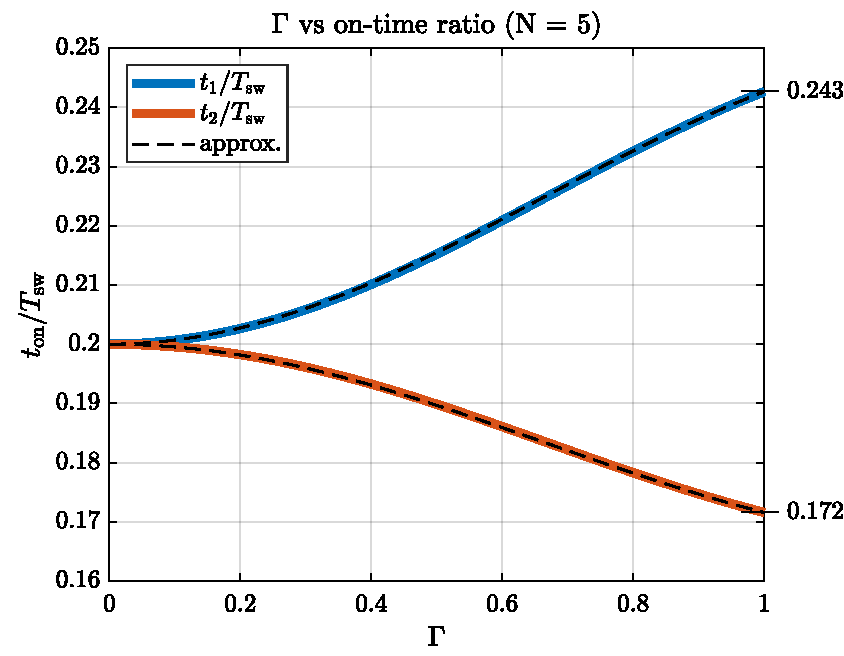
\includegraphics[width=1\linewidth]{Figures/ResonantFCML_Ton_N=5.pdf}
	\caption{Numerical solution of relative phase durations $t_1/T_{\textrm{sw}}$ and $t_2/T_{\textrm{sw}}$ for a 5:1 FCML across $\Gamma$. The closed-form approximations are superimposed with dashed lines.}
	\label{fig:Gamma_vs_Ton}
\end{minipage}
% \hspace{20pt}
\hfill
\begin{minipage}{0.36\linewidth}
    \centering
    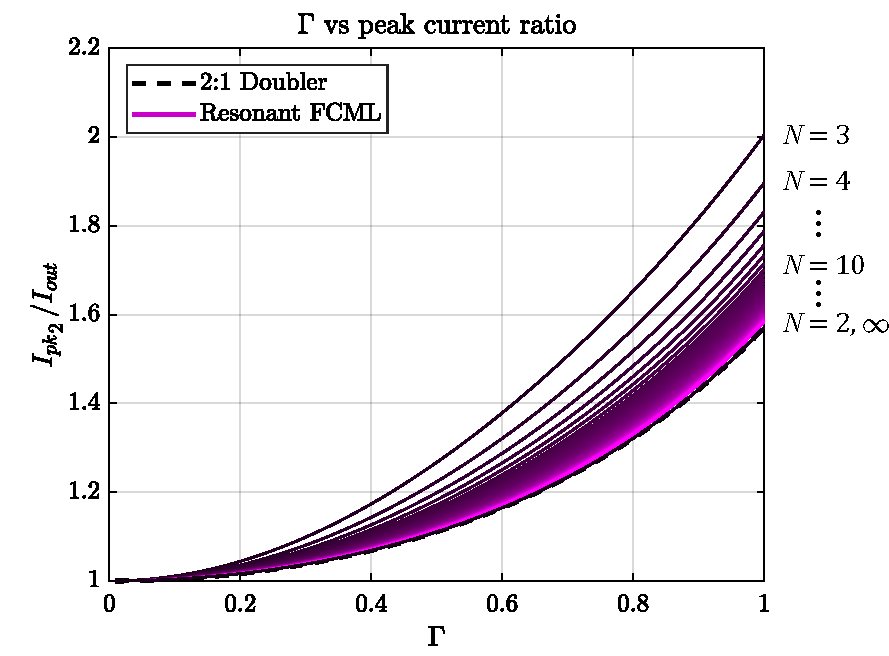
\includegraphics[width=1\linewidth]{Figures/ResonantFCML_IpkIout_b.pdf}
    \caption{$\Gamma$ versus peak-to-average output current $I_{out}$ for all $N$. Peak inductor current occurs during phases 2 to $N$-1, while two flying capacitors are connected in series.}
    \label{fig:ResonantFCML__Gamma_v_IpkIout_all}
\end{minipage}
% \hspace{10pt}
\hfill
\begin{minipage}{0.3\linewidth}
%%%%%%%%%%%%%%%%%%%%%%%%%%%%%%%%%%%%%%%%%%%%%%%%%%%%%%%%%%%%%%%%%%%%%%%%%%%%%%%%%%%%%%%%%%%%%
  \centering
    % 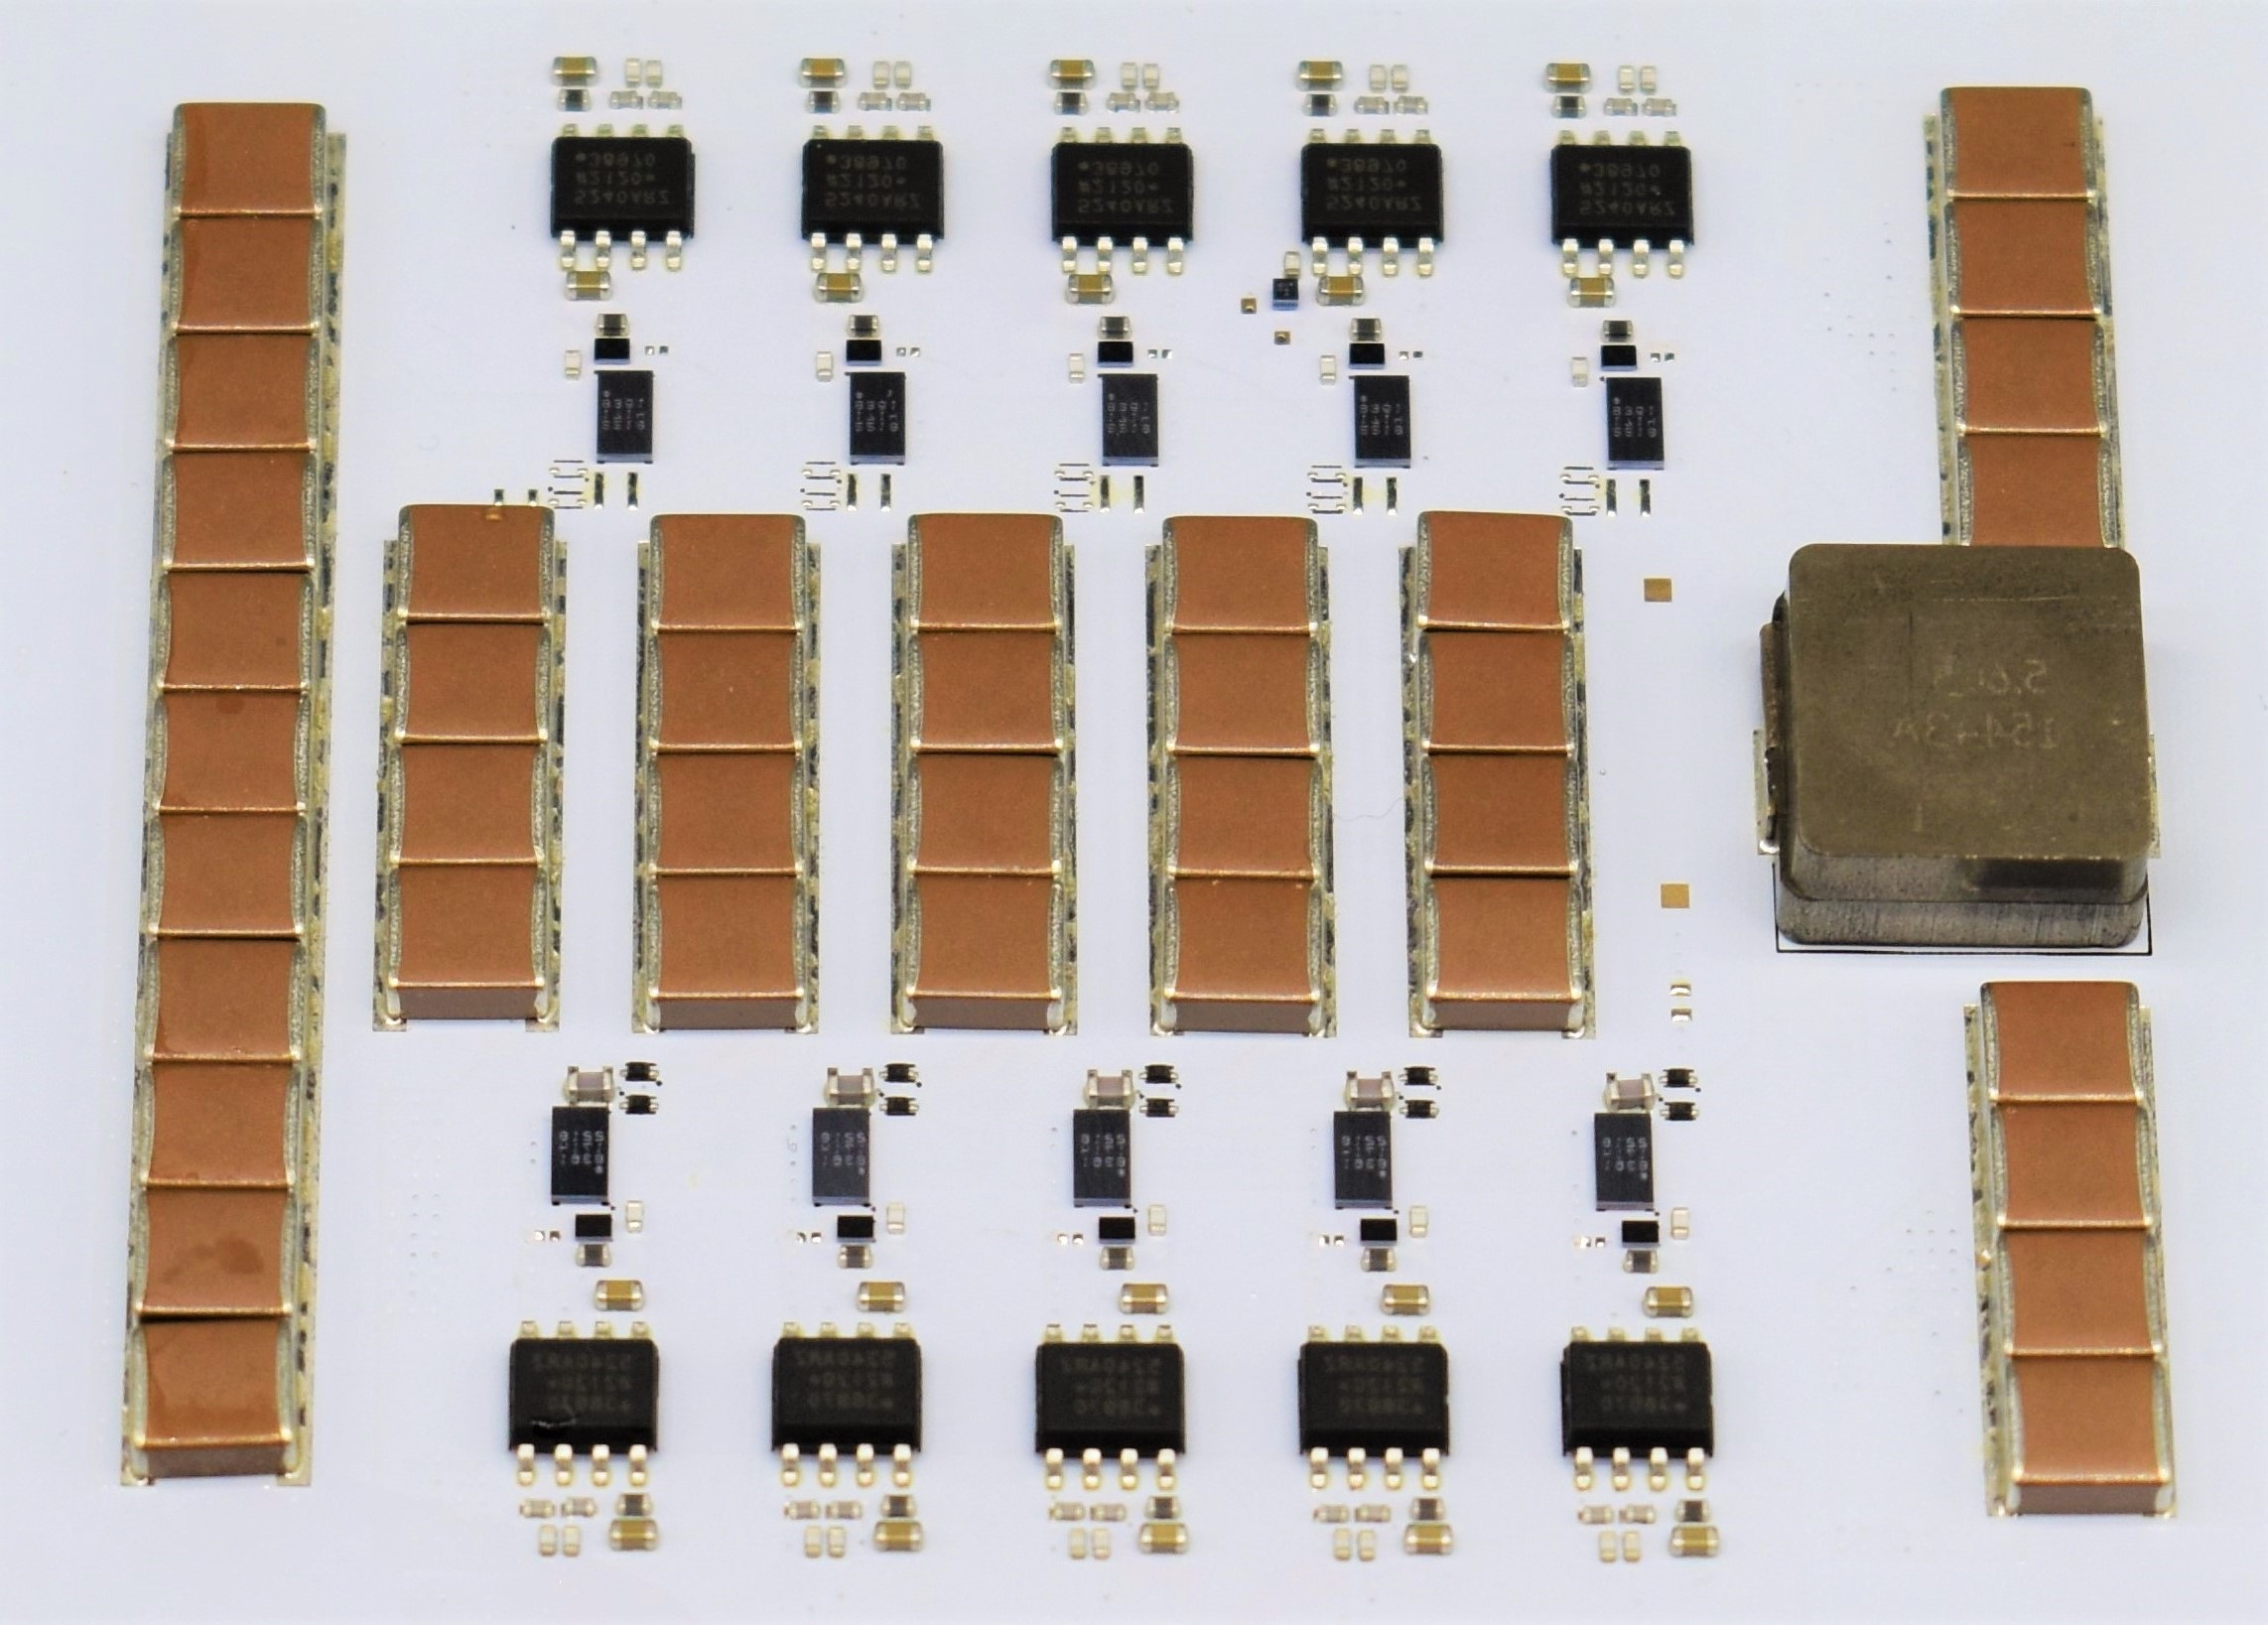
\includegraphics[width=1\linewidth]{Figures/clean_photo_cropped_3.jpg}
    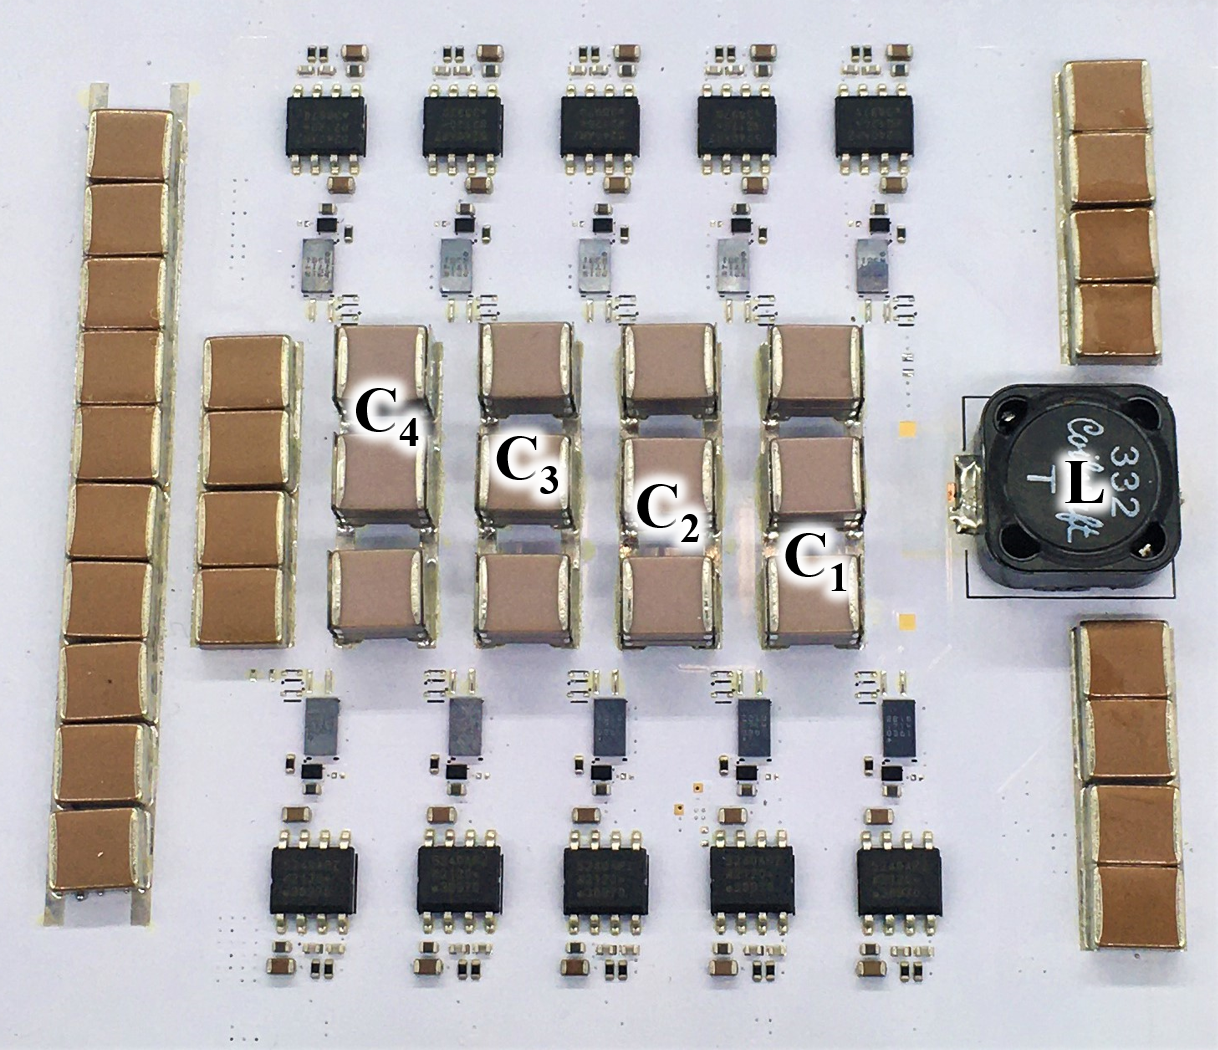
\includegraphics[width=1\linewidth]{Figures/PCB_FCML_annotated.png}
    \caption{Photograph of the constructed 5:1 FCML hardware prototype.}
    \label{fig:board}

%{\renewcommand{\arraystretch}{2.3}
%% \small
%\footnotesize
%% 	\begin{table}[thb]
%		\centering
%% 		\vspace{0.2cm}
%        \captionsetup{type=table} %% tell latex to change to table
%		\caption{Component Details}
%
%		\begin{tabular}{rl}
%            \toprule
%            Component & \makecell[l]{Description \& \\ Part Name} \\
%            \midrule
%            $S_{1\textrm{-}5A}$, $S_{1\textrm{-}5B}$    & \makecell[l]{100\,V, 3.2\,m$\Omega$ GaN-FET \\ EPC2218} \\
%            $C_{1-4}$                                   & \makecell[l]{3 $\times$ 0.3\,$\mu$F, C0G, 250V \\ CKG57NC0G2E304J500JH} %\\
%            $L$                                         & \makecell[l]{3.39\,$\mu$H \\ MSS1260-332NLD} \\
%            $R_{GATE}$                                  & \makecell[l]{37.5\,$\Omega$, 0402 \\ CR0402-16W-35R7FT} \\
%            Gate Driver                                 & \makecell[l]{5\,V, 7\,A\,/\,5\,A \\ LMG1020} \\
%            \makecell[r]{Level-Shift \\ and Power} & ADUM5240\\
%            \bottomrule
%        \end{tabular}
%
%}%


%%%%%%%%%%%%%%%%%%%%%%%%%%%%%%%%%%%%%%%%%%%%%%%%%%%%%%%%%%%%%%%%%%%%%%%%%%%%%%%%%%%%%%%%%%%%%%
\end{minipage}
\vspace{-1.5em}
\end{figure}


From inspection of the numerical solution (an example $N=5$ is shown in Fig.~\ref{fig:Gamma_vs_Ton}), an accurate closed-form expression of the relative phase durations $t_1/T_{\textrm{sw}}$ and $t_2/T_{\textrm{sw}}$ is approximated in (\ref{eqn:t1_approx}) and (\ref{eqn:t2_approx}) as a function of $N$ and $\Gamma$ only.
% \begin{align}
%     t_1 = \Biggl( \biggl(\frac{1}{N} - \frac{\sqrt{2}}{2\sqrt{2}+N-2} \biggr) \cdot \frac{\sin(\pi\Gamma)}{\pi \Gamma} + \frac{\sqrt{2}}{2\sqrt{2}+N-2} \Biggr) \cdot T_{\textrm{sw}} \\
%     t_2 = \Biggl( \biggl(\frac{1}{N} - \frac{1}{2\sqrt{2}+N-2} \biggr) \cdot \frac{\sin(\pi\Gamma)}{\pi \Gamma} + \frac{1}{2\sqrt{2}+N-2} \Biggr) \cdot T_{\textrm{sw}}
% \end{align}

\centerline{
\vspace{10pt}
\begin{tabular}{cc}
    \hspace{-20pt}
    \noindent\parbox[c]{0.55\textwidth}{
    	\begin{equation}
    % 	t_1 \approx \Biggl( \biggl(\frac{1}{N} - \frac{\sqrt{2}}{2\sqrt{2}+N-2} \biggr) \cdot \frac{\sin(\pi\Gamma)}{\pi \Gamma} + \frac{\sqrt{2}}{2\sqrt{2}+N-2} \Biggr) \cdot T_{\textrm{sw}}
    	\frac{t_1}{T_{\textrm{sw}}} \approx \biggl(\frac{1}{N} - \frac{\sqrt{2}}{2\sqrt{2}+N-2} \biggr) \cdot \frac{\sin(\pi\Gamma)}{\pi \Gamma} + \frac{\sqrt{2}}{2\sqrt{2}+N-2}
    	\label{eqn:t1_approx}
    	\end{equation}
    }
    &
    \noindent\parbox[c]{0.55\textwidth}{
    	\begin{equation}
    % 	t_2 \approx \Biggl( \biggl(\frac{1}{N} - \frac{1}{2\sqrt{2}+N-2} \biggr) \cdot \frac{\sin(\pi\Gamma)}{\pi \Gamma} + \frac{1}{2\sqrt{2}+N-2} \Biggr) \cdot T_{\textrm{sw}}
    	\frac{t_2}{T_{\textrm{sw}}} \approx \biggl(\frac{1}{N} - \frac{1}{2\sqrt{2}+N-2} \biggr) \cdot \frac{\sin(\pi\Gamma)}{\pi \Gamma} + \frac{1}{2\sqrt{2}+N-2}
    	\label{eqn:t2_approx}
    	\end{equation}
    }
\end{tabular}
}

\noindent These phase duration approximations can also be used to derive an approximation for the peak-to-average inductor current ratio in (\ref{eqn:I2_Iout})
% \begin{align}
%     % \frac{I_2}{I_{out}} = \frac{ \bigl( \frac{2\sqrt{2}+N-2}{N} \bigr) \cdot \frac{\pi}{2} \Gamma }{\sin\bigl( \frac{\sqrt{2}-1}{N}\sin(\pi\Gamma) + \frac{\pi}{2}\Gamma \bigr) } \\
%     \frac{I_2}{I_{out}} = \frac{ \biggl( \dfrac{2\sqrt{2}+N-2}{N} \biggr) \cdot \dfrac{\pi}{2} \Gamma }{\sin\biggl( \dfrac{\sqrt{2}-1}{N}\sin(\pi\Gamma) + \dfrac{\pi}{2}\Gamma \biggr) }
% \end{align}
which reduces to the precise value in (\ref{eqn:I2_Iout_b}) when at resonance ($\Gamma=1$).
For decreasing $\Gamma$ and increasing $N$ the peak inductor current decreases monotonically, as shown in Fig.~\ref{fig:ResonantFCML__Gamma_v_IpkIout_all}, thus the expected conduction losses also decrease. 

% \begin{equation}
%     \frac{I_2}{I_{out}} = \biggl( \dfrac{2\sqrt{2}+N-2}{N} \biggr) \cdot \dfrac{\pi}{2}
% \end{equation}

\centerline{
% \vspace{20pt}
\begin{tabular}{cc}
    \hspace{-10pt}
    \noindent\parbox[c]{0.5\textwidth}{
    	\begin{equation}
    % 	\frac{I_2}{I_{out}} = \frac{ \biggl( \dfrac{2\sqrt{2}+N-2}{N} \biggr) \cdot \dfrac{\pi}{2} \Gamma }{\sin\biggl( \dfrac{\sqrt{2}-1}{N}\sin(\pi\Gamma) + \dfrac{\pi}{2}\Gamma \biggr) }
        \frac{I_{\textrm{pk}}}{I_{out}} = 
    	\frac{I_{\textrm{pk}_2}}{I_{out}} \approx \frac{ (2\sqrt{2}+N-2 ) \cdot \pi \Gamma }{2N \cdot \sin\biggl( \dfrac{\sqrt{2}-1}{N}\sin(\pi\Gamma) + \dfrac{\pi}{2}\Gamma \biggr) }
    	\label{eqn:I2_Iout}
    	\end{equation}
    }
    &
    \noindent\parbox[c]{0.5\textwidth}{
    % \begin{minipage}{0.55\textwidth}
    	\begin{equation}
    	\frac{I_{\textrm{pk}}}{I_{out}} = \biggl( \dfrac{2\sqrt{2}+N-2}{N} \biggr) \cdot \dfrac{\pi}{2} \qquad \textrm{when $\Gamma=1$}
    	\label{eqn:I2_Iout_b}
    	\end{equation}
% 	\end{minipage}
    }
\end{tabular}
}





	